%% Contoh tesis GayaUKM dalam Bahasa Melayu
\documentclass[bahasam,nohyphen]{GayaUKM}

\usepackage{graphicx}

\title{<Tajuk Tesis Anda, Pecahkan Tajuk Panjang Secara Manual\protect\\Jika Perlu>}
\author{<Nama Anda>}
\authorid{<P00000>}
\faculty{<Fakulti Anda>}
\submissiondate{2 Oktober 2013}
\submissionyear{2013}
\degreetype{Doktor Falsafah}
\campus{Bangi}

%% If you find the boxes around hyperlinks distracting
\hypersetup{colorlinks,allcolors=black}

\begin{document}

%% Cover page
\makecoverpage

%% Re-specify your title with different manual line breaks for the
%% title page, if necessary
\title{<Tajuk Tesis Anda, Pecahkan Tajuk Panjang\protect\\Secara Manual Jika Perlu>}
\maketitlepage

\frontmatter
\declaration

% penghargaan dari penghargaan.tex
\begin{acknowledgements}
Terima kasih kepada sekian yang menawarkan bantuan.
\end{acknowledgements}

% abstrak dlm Bahasa Melayu dari abstrak-ms.tex
\begin{msAbstract}
Inilah abstrak dalam Bahasa Melayu. Data korpus merupakan data bahasa
Melayu yang datangnya dalam dua bentuk sumber, iaitu bentuk tulisan
dan bentuk lisan. Bentuk tulisan seperti buku, majalah, surat khabar,
makalah, monograf, dokumen, kertas kerja, efemeral, puisi, drama,
kad bahan, surat, risalah dan sebagainya. Sementara bentuk lisan yang
ditranskripsikan seperti ucapan, wawancara, temu bual, perbualan dan
sebagainya dalam pelbagai bentuk rakaman.
\end{msAbstract}

% abstrak dlm Bahasa Inggeris dari abstract-en.tex
% Tajuk tesis dalam Bahasa Inggeris perlu diberikan.
\begin{enAbstract}[<Your English Title here>]
This is the English abstract. Auto single-line spacing. Jelly dessert sesame snaps. Oat cake jelly oat cake gingerbread sweet roll apple pie muffin sesame snaps. Dragée icing carrot cake faworki tart chocolate cake. Cookie apple pie chupa chups tootsie roll sweet roll toffee chocolate bar gummies gummi bears. Apple pie lollipop candy canes jujubes caramels. Soufflé powder liquorice fruitcake. Tiramisu fruitcake candy canes jelly beans muffin chupa chups bonbon. Donut sugar plum fruitcake liquorice chocolate pastry lollipop chocolate bar cookie. Jelly-o donut marshmallow chupa chups danish. Sugar plum pudding sweet roll muffin applicake biscuit tart fruitcake wafer. Pudding croissant carrot cake tiramisu candy canes. Powder powder jelly-o. Pie croissant cake chocolate cake carrot cake sweet apple pie sweet roll donut.
\end{enAbstract}


\tableofcontents\clearpage
\listoffigures\clearpage
\listoftables\clearpage

% Senari simbol dll boleh disediakan seperti
% dalam senaraisimbol.tex
\chapter{Senarai Simbol}

%% If your list of symbols/abbreviations are longer than a page, use a
%% longtable or supertabular instead e.g.
%% \begin{longtable}{l@\hspace{...}p{...}}
%% This will require \usepackage{longtable} or \usepackage{supertabular}
%% per your preference

\begin{center}
\doublespacing
\begin{tabular}{l@{\hspace{3em}}p{.6\textwidth}}
$b, c$ & pemalar\\
$C_f$ & pekali geseran kulit setempat\\
\end{tabular}
\end{center}



\mainmatter
% Setiap satu bab dari fail berasingan
\chapter{Pengenalan}
\label{bab:pengenalan}

\section{Pendahuluan}
Teknologi Augmented Reality (AR) telah mengalami evolusi yang signifikan, terutamanya dalam sektor pendidikan, kerana kemampuannya menggabungkan elemen maya dan nyata dalam satu ruang interaktif yang mampu meningkatkan keberkesanan pembelajaran (Azuma, 1997; Wu et al., 2013; Bacca et al., 2014; Billinghurst \& Dünser, 2012). Dalam pendidikan prasekolah, asas literasi dilihat sebagai tunjang utama dalam membentuk kemahiran asas membaca dan menulis yang kritikal untuk perkembangan kognitif kanak-kanak (Mayo, 2019; Jamila et al., 2012). Beberapa kajian menunjukkan bahawa penggunaan pendekatan pembelajaran berasaskan visual, auditori, dan interaktif — seperti yang disokong oleh teknologi AR — dapat memudahkan pemahaman konsep asas huruf serta meningkatkan motivasi dan penglibatan murid (Chen et al., 2020; Rahmawati et al., 2022; Bower et al., 2014; Radu, 2014).
Pendekatan tradisional dalam pendidikan awal, seperti penggunaan buku teks, kad imbas, dan latihan bertulis, masih menjadi pilihan utama di kebanyakan prasekolah. Namun, kurangnya unsur interaktif dalam kaedah konvensional ini sering menyebabkan sebilangan murid menghadapi kesukaran dalam mengenal pasti dan menguasai huruf dengan berkesan (Rahmawati et al., 2022; Jamila et al., 2012). Sebaliknya, aplikasi teknologi AR memberikan peluang pembelajaran yang lebih dinamik dan menyeronokkan dengan membolehkan murid memvisualisasikan huruf dalam bentuk tiga dimensi (3D), mendengar sebutan yang betul, serta berinteraksi dengan animasi yang dapat memperkukuhkan pemahaman konsep (Gunalan et al., 2023; Billinghurst \& Dünser, 2012). Oleh yang demikian, integrasi AR dalam proses pengajaran dan pembelajaran bukan sahaja dapat merangsang minat dan motivasi murid, tetapi juga meningkatkan daya ingatan serta penguasaan literasi awal melalui pendedahan visual, auditori, dan elemen interaktif (UNESCO, 2022; Chen et al., 2020; Radu, 2014).
Kajian ini memfokuskan kepada penilaian keberkesanan aplikasi AR Alphabets dalam membantu murid prasekolah mengenal huruf dengan cara yang lebih menyeronokkan dan interaktif, di samping meneliti kelebihan serta kekurangan penggunaan teknologi ini berbanding pendekatan tradisional seperti buku teks dan latihan bertulis (Kementerian Pendidikan Malaysia, 2015; Gunalan et al., 2023). Melalui integrasi elemen visual, audio, dan animasi dalam aplikasi AR, diharapkan pembelajaran huruf menjadi lebih efektif serta dapat meningkatkan pemahaman dan minat murid (Billinghurst & Dünser, 2012; Wu et al., 2013). Dapatan kajian lepas turut membuktikan bahawa penglibatan aktif murid dalam aktiviti pembelajaran yang menyeronokkan dan interaktif mampu mempercepat penguasaan literasi awal (Mayo, 2019; Bower et al., 2014). Sejajar dengan hasrat untuk memperkasakan pendidikan abad ke-21, Kementerian Pendidikan Malaysia (KPM) turut menyokong penggunaan teknologi inovatif seperti AR di peringkat prasekolah melalui Pelan Pembangunan Pendidikan Malaysia (PPPM) 2013–2025 (Kementerian Pendidikan Malaysia, 2013).
Menurut Kementerian Pendidikan Malaysia (KPM), penggunaan teknologi AR dalam pendidikan prasekolah dapat membantu murid memahami bentuk serta bunyi huruf dengan lebih jelas melalui gabungan visualisasi dan audio yang interaktif. Pendekatan ini juga mampu merangsang perkembangan kemahiran kognitif dan motor halus melalui aktiviti sentuhan serta manipulasi objek digital, selain menggalakkan pembelajaran kendiri di mana kanak-kanak dapat meneroka huruf dalam suasana pembelajaran yang menyeronokkan dan motivasi tinggi (Kementerian Pendidikan Malaysia, 2015; Gunalan et al., 2023). Tambahan pula, laporan UNESCO MGIEP menegaskan bahawa teknologi AR dapat meningkatkan tumpuan dan daya ingatan murid kerana persembahan konsep secara visual dan interaktif mendorong pelajar untuk lebih mudah mengingati serta memahami maklumat (UNESCO, 2022; Bower et al., 2014; Radu, 2014).
Kajian ini bertujuan membangunkan serta menilai aplikasi AR Alphabets dalam konteks pembelajaran prasekolah, di samping meneliti bagaimana teknologi inovatif ini dapat menyokong murid dalam mengenali dan memahami huruf secara lebih berkesan. Kementerian Pendidikan Malaysia (KPM) telah mengambil langkah proaktif dalam mereformasi sistem pendidikan negara, termasuk menerusi pelaksanaan inisiatif seperti Mesyuarat Susulan Jemaah Menteri Bil. 6/2008 dan Pelan Pembangunan Pendidikan Malaysia (PPPM) 2013–2025, yang menekankan kepentingan penggunaan teknologi digital dalam pendidikan (Kementerian Pendidikan Malaysia, 2013). Sejajar dengan tuntutan Revolusi Industri Keempat (IR 4.0), KPM memperkenalkan Pendidikan 4.0 yang memberi fokus kepada penguasaan kemahiran abad ke-21, antaranya pemikiran kritis, kreativiti, penyelesaian masalah dan penerapan pembelajaran berasaskan teknologi (Kementerian Pendidikan Malaysia, 2015; UNESCO, 2022; Gunalan et al., 2023)..
Pengaplikasian teknologi seperti Augmented Reality (AR) semakin diiktiraf sebagai pemangkin pemodenan dalam pendidikan, di mana guru dapat menyampaikan kandungan pengajaran dengan lebih menarik, interaktif, dan efektif. Inisiatif ini selari dengan dasar ICT dalam pendidikan negara yang menekankan penggunaan teknologi digital sebagai strategi meningkatkan kualiti dan akses kepada pembelajaran (Kementerian Pendidikan Malaysia, 2015; Gunalan et al., 2023; Bower et al., 2014). Meskipun terdapat cabaran seperti kos pembangunan aplikasi AR serta keperluan latihan khusus untuk guru, teknologi ini tetap berpotensi besar dalam memperkasakan sistem pendidikan Malaysia agar lebih moden, responsif dan inklusif, selaras dengan aspirasi Pendidikan 4.0 (Gunalan et al., 2023; UNESCO, 2022).
1.2Latar Belakang Kajian
Pembelajaran literasi awal merupakan asas utama dalam perkembangan akademik dan kognitif kanak-kanak, terutamanya bagi murid prasekolah yang sedang belajar mengenali huruf dan perkataan (Mayo, 2019; Zhou et al., 2021). Kajian menunjukkan bahawa kemahiran membaca dan menulis yang kukuh di peringkat prasekolah berkait rapat dengan prestasi akademik di sekolah rendah dan seterusnya (Zhou et al., 2021).
Pendekatan tradisional dalam pembelajaran huruf, seperti penggunaan buku teks, kad imbas, dan kaedah pengulangan, masih digunakan dalam sistem pendidikan. Walau bagaimanapun, kaedah ini mungkin kurang menarik bagi murid prasekolah dan boleh menyebabkan mereka hilang fokus semasa belajar (Chen et al., 2020). Oleh itu, integrasi teknologi seperti Augmented Reality (AR) menawarkan pendekatan pembelajaran yang lebih interaktif dan sesuai dengan perkembangan digital dalam pendidikan awal kanak-kanak.
Teknologi AR membolehkan pengguna berinteraksi dengan objek digital dalam dunia nyata, menjadikan pengalaman pembelajaran lebih visual, dinamik, dan menarik (Azuma, 1997). Kajian telah menunjukkan bahawa penggunaan AR dalam pendidikan mampu meningkatkan pemahaman murid, motivasi, dan daya ingatan, serta membolehkan mereka mengalami konsep pembelajaran dengan lebih realistik (Wu et al., 2013).
Kajian oleh Billinghurst dan Dünser (2012) mendapati bahawa murid yang belajar menggunakan modul interaktif berasaskan AR mampu mengingati konsep dengan lebih cepat berbanding mereka yang menggunakan bahan pembelajaran tradisional. Sementara itu, Rahmawati et al. (2022) menunjukkan bahawa AR dapat membantu kanak-kanak mengenali huruf dengan lebih efektif melalui penggunaan model 3D dan kesan animasi.Di Malaysia, KPM menggalakkan penggunaan AR dalam pendidikan prasekolah, selaras dengan usaha memperkukuh literasi digital generasi muda (KPM, 2013).
Penggunaan AR dalam Pendidikan Prasekolah di Malaysia
Di Malaysia, Kementerian Pendidikan Malaysia (KPM) telah menggalakkan penggunaan teknologi digital dalam pendidikan prasekolah, termasuk elemen gamifikasi, AR, dan multimedia interaktif, sejajar dengan Pelan Pembangunan Pendidikan Malaysia (PPPM) 2013–2025.
Menurut laporan KPM, penggunaan AR dalam pendidikan prasekolah boleh membantu murid untuk memahami bentuk dan bunyi huruf dengan lebih jelas melalui visualisasi dan audio interaktif, meningkatkan kemahiran kognitif dan motor halus dengan aktiviti sentuhan serta manipulasi objek huruf dalam AR, serta menggalakkan pembelajaran kendiri yang membolehkan kanak-kanak meneroka huruf secara lebih menyeronokkan.
Selain itu, laporan UNESCO MGIEP menyatakan bahawa teknologi AR dapat meningkatkan tumpuan dan daya ingatan pelajar, kerana mereka lebih cenderung mengingati sesuatu konsep apabila ia dipersembahkan dalam bentuk visual dan interaktif (UNESCO, 2022).
Fokus Kajian
Berdasarkan maklumat di atas, kajian ini akan membangunkan dan menilai keberkesanan aplikasi AR Alphabets dalam membantu murid prasekolah mengenali huruf dengan pendekatan yang lebih interaktif dan menyeronokkan.
Kajian ini juga akan menggunakan pengujian kebolehgunaan seperti System Usability Scale (SUS) untuk menilai kemudahan penggunaan aplikasi serta pengalaman pengguna.
1.3Pernyataan Masalah
Pembelajaran literasi awal merupakan asas penting dalam pendidikan prasekolah kerana ia membantu kanak-kanak mengenali huruf, memahami bunyi, dan mengembangkan kemahiran membaca. Walaupun terdapat pelbagai inovasi teknologi pendidikan, kaedah konvensional masih menjadi pilihan utama di peringkat prasekolah. Kajian menunjukkan murid prasekolah menghadapi cabaran dalam pembelajaran literasi disebabkan kekurangan elemen interaktif dan motivasi yang rendah (Rahmawati et al., 2022; Zhou et al., 2021).
Guru juga menghadapi keterbatasan dari segi latihan penggunaan teknologi seperti AR (UNESCO, 2022). Justeru, pembangunan aplikasi AR Alphabets ini diharap dapat menambah nilai dan meningkatkan keberkesanan pembelajaran literasi awa.
Beberapa isu utama yang dikenal pasti dalam pembelajaran huruf bagi kanak-kanak prasekolah adalah seperti berikut:
1.Kurangnya elemen interaktif dalam pembelajaran huruf.
2.Motivasi pembelajaran yang rendah dalam kalangan murid prasekolah.
3.Kesukaran mengingat bentuk dan bunyi huruf, terutama bagi huruf yang mempunyai bentuk hampir serupa (contoh: “b” dan “d”).
4.Keterbatasan guru dalam menerapkan teknologi pendidikan, kerana tidak semua guru diberi latihan yang mencukupi untuk menggunakan alat pembelajaran digital seperti AR (UNESCO, 2022).
Kajian menunjukkan bahawa kaedah pembelajaran berasaskan visual dan auditori dapat membantu meningkatkan kefahaman murid (Billinghurst & Dünser, 2012). Murid prasekolah sering menghadapi cabaran dalam mengenal pasti bentuk huruf serta mengingati bunyi huruf dengan betul. Selain itu, kajian mendapati bahawa pelajar lebih cenderung untuk hilang fokus dalam pembelajaran huruf apabila tiada elemen interaktif dan menarik, menyebabkan mereka lambat dalam proses pengecaman huruf dan sebutan (Rahmawati et al., 2022).
Sebagai penyelesaian kepada masalah ini, teknologi Augmented Reality (AR) menawarkan pendekatan pembelajaran yang lebih visual, interaktif, dan menarik. AR dapat membantu murid prasekolah melihat, mendengar, dan berinteraksi dengan huruf dalam bentuk 3D, menjadikan pengalaman pembelajaran lebih menyeronokkan dan mudah difahami.
Kajian ini bertujuan untuk menilai keberkesanan aplikasi AR Alphabets dalam meningkatkan pengalaman pembelajaran huruf bagi murid prasekolah, serta mengenal pasti keuntungan dan cabaran teknologi ini berbanding kaedah pembelajaran tradisional. Murid prasekolah cenderung belajar dengan menggunakan deria mereka, namun kaedah pembelajaran tradisional kurang menawarkan visualisasi dinamik, animasi, dan elemen auditori yang dapat membantu mereka mengenali huruf dengan lebih berkesan (Chen et al., 2020).
1.4Objektif Kajian
Kajian ini bertujuan untuk:
1.Mengkaji pencapaian murid setelah menjalani proses pembelajaran menggunakan aplikasi AR Alphabets, khususnya dalam pengenalan huruf dan pemahaman fonetik. 
2.Menilai perubahan pemahaman murid sebelum dan selepas penggunaan AR Alphabets, bagi mengenal pasti sejauh mana aplikasi ini membantu murid memahami huruf secara lebih berkesan melalui elemen interaktif seperti audio dan animasi 3D.
3.Menganalisis perubahan daya tumpuan murid selepas proses pembelajaran menggunakan AR Alphabets, dan penerimaan pengguna terhadap aplikasi AR Alphabets

1.5Soalan Kajian
Persoalan kajian adalah seperti berikut :
1.Adakah terdapat peningkatan prestasi pencapaian murid setelah menjalani proses pembelajaran menggunakan aplikasi AR Alphabets?
2.Adakah terdapat perubahan dalam pemahaman murid setelah melalui proses pembelajaran menggunakan AR Alphabets, khususnya dalam mengenal huruf dan memahami fonetik?
3.Adakah terdapat perubahan dalam tumpuan murid selepas menggunakan AR Alphabets, dan apakah tahap penerimaan guru dan murid terhadap AR Alphabets ?

1.6Batasan Kajian
Kajian ini menumpukan kepada penggunaan aplikasi AR Alphabets dalam pembelajaran literasi awal bagi murid prasekolah di sebuah institusi pendidikan prasekolah yang dipilih.
Struktur organisasi prasekolah yang menjadi tempat kajian terdiri daripada seorang guru besar, seorang penolong kanan pentadbiran, seorang penolong kanan hal ehwal murid, dan seorang penolong kanan kokurikulum. Institusi tersebut mempunyai jumlah keseluruhan murid prasekolah, dengan sekumpulan murid yang dipilih sebagai sampel kajian berdasarkan pengalaman mereka dalam pembelajaran literasi awal.
Kajian ini tidak melibatkan murid pendidikan khas, tetapi memberi tumpuan kepada murid prasekolah yang mengikuti kurikulum biasa, khususnya dalam pembelajaran mengenal huruf dan memahami bunyi fonetik menggunakan teknologi Augmented Reality (AR).
Saiz sampel kajian terdiri daripada sekumpulan murid prasekolah yang dipilih berdasarkan interaksi mereka dengan AR Alphabets, bagi menilai impak aplikasi terhadap pemahaman huruf, daya tumpuan, dan motivasi pembelajaran mereka.
Kajian ini terhad kepada satu institusi prasekolah, dan penemuan yang diperoleh akan memberi gambaran tentang keberkesanan AR dalam pendidikan awal, namun tidak boleh digeneralisasikan kepada semua sekolah prasekolah di Malaysia tanpa kajian lanjut.
1.7 Kepentingan Kajian
Kajian ini mempunyai kepentingan yang besar dalam bidang pendidikan prasekolah, khususnya dalam pembelajaran literasi awal menggunakan teknologi Augmented Reality (AR).
1.7.1 Kepentingan kepada Murid Prasekolah
Meningkatkan pemahaman dan daya ingatan murid terhadap bentuk dan bunyi huruf melalui visualisasi interaktif.  Menggalakkan pembelajaran kendiri, membolehkan murid berinteraksi dengan huruf dalam bentuk 3D dan memahami konsep secara aktif. Menjadikan pembelajaran lebih menyeronokkan dan menarik, membantu meningkatkan motivasi murid dalam mengenali huruf dengan lebih cepat.(Wu et al., 2013)
1.7.2 Kepentingan kepada Guru
Membantu guru dalam menyampaikan pelajaran dengan lebih efektif, menggunakan animasi 3D dan bunyi sebutan huruf. Menyediakan alat bantu mengajar yang inovatif, yang boleh digunakan untuk meningkatkan keberkesanan pengajaran literasi awal. (Gunalan et al., 2023)Memudahkan guru mengenal pasti kesulitan murid dalam pembelajaran huruf, dengan adanya sistem interaktif dan maklum balas digital.
1.7.3Kepentingan kepada Sistem Pendidikan
Menyokong Pelan Pembangunan Pendidikan Malaysia (PPPM) 2013-2025, yang menggalakkan penggunaan teknologi dalam pendidikan. Membantu memperkaya kurikulum pendidikan prasekolah, dengan mengintegrasikan teknologi digital dan pembelajaran interaktif. (KPM, 2013; UNESCO, 2022)Menjadi rujukan kepada kajian teknologi pendidikan, khususnya dalam pengembangan aplikasi pembelajaran berbasis AR bagi kanak-kanak.
1.7.4 Kepentingan kepada Penyelidikan Teknologi
Menyumbang kepada inovasi teknologi pendidikan, dengan membangunkan aplikasi AR Alphabets yang lebih mesra pengguna (Bacca et al., 2014). Membantu dalam memahami keberkesanan AR dalam literasi awal, dengan menggunakan metodologi pengujian usability seperti System Usability Scale (SUS). Menjadi asas kepada kajian lanjut dalam bidang AR, khususnya dalam pembangunan aplikasi pendidikan interaktif untuk murid prasekolah.
1.8Definisi Operasi
1.8.1Augmented Reality (AR)
Definisi Umum: Teknologi yang menggabungkan elemen digital ke dalam dunia nyata, membolehkan pengguna berinteraksi dengan objek maya dalam persekitaran fizikal  (Azuma, 1997; Wu et al., 2013). Definisi Operasi dalam Kajian Ini: AR digunakan dalam aplikasi AR Alphabets untuk membantu murid prasekolah melihat, mendengar, dan berinteraksi dengan huruf dalam bentuk 3D bagi meningkatkan pemahaman mereka terhadap literasi awal.
1.8.2Literasi Awal
Definisi Umum: Keupayaan kanak-kanak untuk mengenali huruf, memahami bunyi, dan mengembangkan kemahiran membaca serta menulis (Mayo, 2019). Definisi Operasi dalam Kajian Ini: Literasi awal merujuk kepada kemampuan murid prasekolah mengenali dan mengingat bentuk serta bunyi huruf, yang diuji melalui penggunaan aplikasi AR Alphabets.
1.8.3Murid Prasekolah
Definisi Umum: Kanak-kanak berusia 4 hingga 6 tahun yang berada dalam fasa pendidikan awal sebelum memasuki sekolah rendah (UNESCO, 2022). �� Definisi Operasi dalam Kajian Ini: Murid prasekolah yang terlibat dalam kajian ini berusia 5 hingga 6 tahun, di mana mereka diuji untuk melihat keberkesanan penggunaan AR dalam pembelajaran huruf.
1.8.4Aplikasi Pembelajaran
Aplikasi pembelajaran ialah perisian yang dibangunkan untuk menyokong proses pengajaran dan pembelajaran (PdP). Dalam kajian ini, aplikasi AR Alphabets dibangunkan sebagai bahan bantu mengajar (BBM) dalam pembelajaran literasi awal, membolehkan murid mengimbas kad huruf dan melihat animasi interaktif sebagai sebahagian daripada kaedah pembelajaran digital yang lebih menarik.
1.8.5Pencapaian
Pencapaian akademik dalam kajian ini merujuk kepada kemampuan murid mengenal huruf dan memahami fonetik selepas menggunakan AR Alphabets. Kajian menilai kemajuan murid melalui ujian pra dan ujian pasca, bagi melihat sejauh mana aplikasi ini membantu mereka mengenal pasti huruf dengan lebih berkesan.
1.8.6 Pemahaman
Pemahaman dalam konteks kajian ini ialah keupayaan murid untuk mengenali huruf dan memahami bunyi fonetik dengan lebih mendalam, berdasarkan visualisasi yang diberikan dalam aplikasi AR Alphabets.
1.8.7Tumpuan
Tumpuan merujuk kepada kemampuan murid untuk memberi perhatian dalam proses pembelajaran. Kajian ini mengkaji sejauh mana AR Alphabets membantu meningkatkan daya fokus murid terhadap literasi awal, berbanding kaedah pengajaran tradisional yang kurang interaktif.



?}
\label{sec:apadia}

Lorem Ipsum adalah contoh teks atau dummy dalam industri percetakan dan penataan huruf atau typesetting. Lorem Ipsum telah menjadi standar contoh teks sejak tahun 1500an, saat seorang tukang cetak yang tidak dikenal mengambil sebuah kumpulan teks dan mengacaknya untuk menjadi sebuah buku contoh huruf \cite{banerjee:pedersen:2003}. Ia tidak hanya bertahan selama 5 abad, tapi juga telah beralih ke penataan huruf elektronik, tanpa ada perubahan apapun. Ia mulai dipopulerkan pada tahun 1960 dengan diluncurkannya lembaran-lembaran Letraset yang menggunakan kalimat-kalimat dari Lorem Ipsum, dan seiring munculnya perangkat lunak Desktop Publishing seperti Aldus PageMaker juga memiliki versi Lorem Ipsum \cite{berment:phd:2004}.



\section{Dari Mana Asalnya?}
\label{sec:asal}

\begin{equation}
C_p = \frac{P - P_\infty}{\frac{1}{2} \rho {U_\infty}^2}
 = 1 - \left( \frac{U_1}{U_\infty} \right)^2,
\end{equation}

Tidak seperti anggapan banyak orang, Lorem Ipsum bukanlah teks-teks yang diacak. Ia berakar dari sebuah naskah sastra latin klasik dari era 45 sebelum masehi, hingga bisa dipastikan usianya telah mencapai lebih dari 2000 tahun. Richard McClintock, seorang professor Bahasa Latin dari Hampden-Sidney College di Virginia, mencoba mencari makna salah satu kata latin yang dianggap paling tidak jelas, yakni consectetur, yang diambil dari salah satu bagian Lorem Ipsum. Setelah ia mencari maknanya di di literatur klasik, ia mendapatkan sebuah sumber yang tidak bisa diragukan. Lorem Ipsum berasal dari bagian 1.10.32 dan 1.10.33 dari naskah ``de Finibus Bonorum et Malorum'' (Sisi Ekstrim dari Kebaikan dan Kejahatan) karya Cicero, yang ditulis pada tahun 45 sebelum masehi \cite{azarova:etal:2002,budanitsky:hirst:2006}. Buku ini adalah risalah dari teori etika yang sangat terkenal pada masa Renaissance. Baris pertama dari Lorem Ipsum, ``Lorem ipsum dolor sit amet\ldots'', berasal dari sebuah baris di bagian 1.10.32.

Bagian standar dari teks Lorem Ipsum yang digunakan sejak tahun 1500an kini di reproduksi kembali di bawah ini untuk mereka yang tertarik. Bagian 1.10.32 dan 1.10.33 dari "de Finibus Bonorum et Malorum" karya Cicero juga di reproduksi persis seperti bentuk aslinya, diikuti oleh versi bahasa Inggris yang berasal dari terjemahan tahun 1914 oleh H. Rackham.

\begin{equation}
-\frac{(x_0 - \mu)^2}{2 \sigma^2} = -\ln 2
\end{equation}


\section{Contoh}
\label{sec:contol}

Perenggan awal Lorem Ipsum seperti di bawah.

\subsection{Perenggan Pertama}

Lorem ipsum dolor sit amet, consectetur adipiscing elit. Donec posuere, neque quis feugiat egestas, quam sapien dictum justo, eu vulputate nunc metus sed dui. Integer molestie leo quis libero facilisis, dictum pretium quam ornare. Vestibulum ante ipsum primis in faucibus orci luctus et ultrices posuere cubilia Curae; Vivamus luctus rutrum magna non convallis. Praesent vestibulum consequat eros, et fringilla nisi suscipit id. Nam vulputate justo dui, eu rutrum est accumsan ut. Sed molestie erat vitae mi blandit, in volutpat urna lobortis. Vestibulum mollis rutrum gravida. Fusce dolor nulla, condimentum vel pretium ut, venenatis eget leo. Ut semper placerat mauris, ut tempus est tempor vel. Interdum et malesuada fames ac ante ipsum primis in faucibus. In vitae feugiat diam. Pellentesque accumsan consequat turpis aliquam elementum.


\subsection{Dua Perenggan Seterusnya}

Vivamus dignissim arcu nunc, non aliquam sem porta vitae. Sed sodales accumsan dui sit amet egestas. Maecenas rhoncus a erat eget accumsan.

\begin{table}[hbt!]\centering
\caption{Bilangan permata}

\begin{tabular}{l c}
\hline
Jenis & Bilangan \\\hline
Nilam & 6\\
Berlian & 23\\
Emas & 56\\
Perak & 235\\
Gangsa & 324\\\hline
\end{tabular}
\end{table}

\begin{itemize}
\item Etiam vitae pulvinar metus, sed fringilla orci.
\item Duis dapibus dolor risus, non ultrices enim porta sit amet.
\item Ut eu libero augue.
\end{itemize}

Nulla ipsum augue, feugiat ac laoreet quis, pretium ut magna. Class aptent taciti sociosqu ad litora torquent per conubia nostra, per inceptos himenaeos. Integer blandit placerat dictum.

\begin{figure}[hbt!]\centering

\includegraphics[width=.5\textwidth]{green}
\caption{Contoh rajah}
\end{figure}

Sed dolor justo, scelerisque sed rutrum quis, porttitor a mauris. Cras non auctor felis, rutrum fringilla risus. Integer at convallis erat, sit amet luctus turpis. Duis sed rutrum eros, quis tempus risus. Etiam pellentesque nisi odio, eget dignissim eros ultrices et. Aliquam leo massa, fermentum vel odio sed, ullamcorper molestie lorem. Integer lorem felis, adipiscing sit amet interdum eget, auctor at lorem. Aliquam ultricies tortor eu nibh facilisis tincidunt.


\subsubsection{Sedikit Catatan}

Duis sed rutrum eros, quis tempus risus. Etiam pellentesque nisi odio, eget dignissim eros ultrices et. Aliquam leo massa, fermentum vel odio sed, ullamcorper molestie lorem.

\subsubsection{Selanjutnya}
Duis sed rutrum eros, quis tempus risus. Etiam pellentesque nisi odio, eget dignissim eros ultrices et. Aliquam leo massa, fermentum vel odio sed, ullamcorper molestie lorem.


\section{Ringkasan}
Nulla ipsum augue, feugiat ac laoreet quis, pretium ut magna. Class aptent taciti sociosqu ad litora torquent per conubia nostra, per inceptos himenaeos. Integer blandit placerat dictum.

Sed dolor justo, scelerisque sed rutrum quis, porttitor a mauris. Cras non auctor felis, rutrum fringilla risus. Integer at convallis erat, sit amet luctus turpis. Duis sed rutrum eros, quis tempus risus. Etiam pellentesque nisi odio, eget dignissim eros ultrices et. Aliquam leo massa, fermentum vel odio sed, ullamcorper molestie lorem. Integer lorem felis, adipiscing sit amet interdum eget, auctor at lorem. Aliquam ultricies tortor eu nibh facilisis tincidunt.

\chapter{LITERATURE REVIEW}                                       

\section{Pengenalan}

Bab ini membincangkan konsep literasi dalam konteks pendidikan prasekolah serta potensi penggunaan Augmented Reality (AR) sebagai alat inovatif untuk memperkayakan pengalaman pembelajaran huruf dalam kalangan murid prasekolah. Kajian lampau telah menunjukkan bahawa meskipun kaedah pembelajaran tradisional seperti buku teks dan latihan bertulis masih meluas digunakan, ia menghadapi pelbagai cabaran dalam memastikan murid benar-benar menguasai, mengingati dan berinteraksi dengan konsep literasi secara menyeluruh (Gee, 1999; Jamila et al., 2012). Seiring perkembangan teknologi dan permintaan pendidikan abad ke-21, integrasi teknologi seperti AR dalam literasi awal semakin menjadi tumpuan dalam bidang akademik dan amalan pendidikan, memandangkan potensinya untuk menyediakan pendekatan yang lebih interaktif, menyeronokkan, serta efektif dalam pembelajaran huruf dan kemahiran membaca (Azuma, 1997; Bacca et al., 2014; Chen et al., 2020; Radu, 2014).

\section{Teori New Literacy Studies (NLS)}
2.2.1Pengenalan kepada NLS
Dalam era pendidikan moden, literasi tidak lagi terhad kepada kemahiran membaca dan menulis secara mekanikal semata-mata, tetapi telah berkembang menjadi satu amalan sosial dan budaya yang dipengaruhi oleh kemajuan teknologi, interaksi antara individu, serta perkembangan dunia digital (Gee, 1999; Kementerian Pendidikan Malaysia, 2013; Bower et al., 2014). Perubahan ini menuntut murid untuk bukan sahaja menguasai literasi asas, tetapi juga kebolehan menggunakan teknologi dan berinteraksi dalam pelbagai konteks pembelajaran abad ke-21 (UNESCO, 2022)
James Paul Gee (1999) merupakan salah seorang sarjana yang memperkenalkan New Literacy Studies (NLS), yang menekankan bahawa literasi bukan hanya merujuk kepada keupayaan membaca dan menulis secara formal, tetapi juga bagaimana seseorang menggunakan bahasa dan komunikasi dalam situasi sosial yang lebih luas.


Street (2003) pula memperkukuhkan konsep ini dengan menyatakan bahawa literasi bukan sekadar kecekapan kognitif, tetapi turut berkait rapat dengan budaya, masyarakat, dan teknologi. Kajian NLS menunjukkan bahawa literasi berkembang mengikut keperluan sosial, di mana seseorang bukan hanya memahami perkataan, tetapi juga menggunakannya, menyesuaikan diri, serta berinteraksi dengan maklumat dalam konteks dunia sebenar.
\section{Implikasi NLS dalam Pendidikan Moden}
Teknologi Augmented Reality (AR) memainkan peranan penting dalam mengukuhkan pendekatan New Literacy Studies, kerana ia mengubah cara pelajar berinteraksi dengan bahan pembelajaran.
Pembelajaran huruf tidak lagi terbatas kepada format dua dimensi (2D) yang statik, tetapi telah berkembang kepada bentuk tiga dimensi (3D) yang lebih interaktif. Dengan teknologi AR, pelajar dapat melihat, menyentuh, dan mendengar huruf serta perkataan dalam cara yang lebih dinamik, seterusnya membantu mereka memahami konsep dengan lebih mendalam.
Tambahan pula, AR membolehkan murid memahami bukan sahaja bentuk huruf, tetapi juga cara huruf digunakan dalam kehidupan sebenar melalui visualisasi dan animasi. Pendekatan ini selari dengan konsep NLS, yang menekankan bahawa literasi moden bukan sekadar kemahiran teknikal, tetapi turut diperkaya dengan konteks sosial dan teknologi.
\section{Kajian Terdahulu Mengenai NLS dan AR dalam Pendidikan}
Beberapa kajian terdahulu telah membuktikan hubungan antara New Literacy Studies dan penggunaan AR dalam pendidikan, seperti yang ditunjukkan dalam Jadual 2.1:
Jadual  2-1 Hubungan antara New Literacy Studies dan penggunaanAR dalam pendidikan


\documentclass{article}
\usepackage{longtable}
\usepackage{lscape}
\usepackage[margin=2.5cm]{geometry}
\renewcommand{\arraystretch}{1.2}
\usepackage{array}

\begin{document}
\begin{landscape}

\begin{longtable}{|p{4.5cm}|p{4.5cm}|p{5cm}|p{4cm}|p{6cm}|}
\caption{Gabungan Kajian AR dalam Pendidikan} \label{tab:kajian_ar} \\
\hline
\textbf{Pengkaji dan Tahun} & \textbf{Fokus Kajian} & \textbf{Kaedah Kajian} & \textbf{Saiz Sampel / Bilangan Kajian} & \textbf{Dapatan Utama} \\
\hline
\endfirsthead
\hline
\textbf{Pengkaji dan Tahun} & \textbf{Fokus Kajian} & \textbf{Kaedah Kajian} & \textbf{Saiz Sampel / Bilangan Kajian} & \textbf{Dapatan Utama} \\
\hline
\endhead
Billinghurst \& Duenser (2012) & Kesan AR dalam pendidikan & Kajian kes buku AR dan aplikasi mudah alih & Tidak dinyatakan & AR meningkatkan daya ingatan dan kefahaman \\
\hline
Luo et al. (2018) & Alat AR untuk kejuruteraan pembinaan & Kajian kes dengan soal selidik dan temu bual & 40 pelajar & Hasil pembelajaran dan visualisasi lebih baik berbanding kaedah 2D \\
\hline
Kaur et al. (2020) & AR untuk pembelajaran interaktif & Intervensi bilik darjah dan soal selidik model ARCS & 34 pelajar & AR tingkatkan motivasi dan kaedah eksplorasi konsep \\
\hline
Tuli et al. (2020) & AR dalam pendidikan sains dan kejuruteraan & Ujian pra-pasca dan analisis prestasi pelajar & Pelajar sekolah menengah dan kejuruteraan & AR bantu pemahaman elektromagnet dan sebagai makmal maya \\
\hline
Jesionkowska et al. (2020) & AR dalam pendidikan STEAM & Pembelajaran berasaskan projek dengan Unity dan HoloLens & 19 peserta (guru dan pelajar) & AR tingkatkan motivasi dan pembangunan kemahiran \\
\hline
Fitria et al. (2023) & Simulasi AR dalam kejuruteraan mekanikal & Kuasi-eksperimen dengan ujian pra dan pasca & 70 pelajar & AR bantu kefahaman dan kemahiran amali pelajar \\
\hline
\end{longtable}

\end{landscape}
\end{document}




2.4.1Implikasi kepada Kajian Ini
Kajian ini menerapkan prinsip New Literacy Studies (NLS) melalui pembangunan aplikasi AR Alphabets, bagi menilai bagaimana teknologi ini dapat membantu meningkatkan literasi awal murid prasekolah secara interaktif dan visual.
Teknologi Augmented Reality (AR) berfungsi sebagai pelengkap kepada pendekatan NLS, membolehkan murid berinteraksi dengan huruf dan bunyi dalam bentuk yang lebih menarik dan berkesan. Kajian ini akan membandingkan keberkesanan AR dengan kaedah pembelajaran tradisional, sejajar dengan pandangan NLS yang menekankan bahawa literasi moden perlu berkembang selaras dengan perubahan teknologi.
2.4.2Kesimpulan
Bab ini telah mengembangkan Teori New Literacy Studies (NLS) secara lebih mendalam dan kritikal, menjelaskan bahawa literasi bukan sekadar kemahiran membaca dan menulis, tetapi juga praktik sosial yang diperkaya dengan teknologi seperti AR.
Kajian ini akan meneliti bagaimana integrasi AR dapat memperkukuhkan pembelajaran literasi awal, memberikan pengalaman pembelajaran yang lebih dinamik, interaktif, dan efektif bagi murid prasekolah.
Multiliteracies dan Literasi Digital
Dalam dunia pendidikan moden, konsep literasi tidak lagi terbatas kepada bacaan dan penulisan dalam bentuk teks sahaja, tetapi telah berkembang kepada pelbagai bentuk komunikasi yang lebih luas dan kompleks.
Kalantzis dan Cope (2000) memperkenalkan konsep Multiliteracies, yang memberi tumpuan kepada cara manusia berkomunikasi melalui pelbagai saluran, termasuk visual, auditori, digital, dan multimodal. Konsep ini berkembang selaras dengan perubahan dalam cara maklumat disampaikan dan diterima oleh masyarakat moden.
Dengan kepesatan teknologi dan globalisasi, pembelajaran tidak lagi tertumpu kepada buku teks dan tulisan sahaja, tetapi merangkumi pelbagai medium komunikasi digital, seperti grafik, video, animasi, dan interaksi teknologi.
Pendekatan Multiliteracies menekankan bahawa pelajar tidak hanya berinteraksi dengan teks bertulis, tetapi juga dengan imej, bunyi, animasi, serta teknologi digital, yang menjadi sebahagian daripada pengalaman pembelajaran mereka. Dalam dunia yang dipenuhi dengan maklumat digital, pelajar perlu menguasai bukan sahaja literasi tradisional, tetapi juga kemahiran teknologi untuk memahami dan memproses maklumat dengan lebih efektif dan efisien.
2.5.1Multiliteracies dan Literasi Digital dalam Konteks Pendidikan
Literasi digital merujuk kepada keupayaan seseorang dalam memahami, menilai, dan menggunakan teknologi untuk mengakses dan menganalisis maklumat (UNESCO, 2022).
Dalam sistem pendidikan yang semakin bergantung kepada teknologi, pelajar perlu menguasai kemahiran digital bagi memahami dunia yang semakin pantas dan interaktif. Kajian menunjukkan bahawa pelajar yang mempunyai literasi digital yang tinggi lebih cenderung untuk memahami konsep pembelajaran dengan lebih mendalam dan mampu menyesuaikan diri dengan pelbagai bentuk komunikasi (Buckingham, 2008).
Teknologi seperti Augmented Reality (AR) dan Virtual Reality (VR) kini digunakan untuk memperkukuhkan literasi digital, dengan membolehkan pelajar berinteraksi dengan konsep pembelajaran dalam persekitaran maya yang lebih realistik (Billinghurst & Dünser, 2012).
Sebagai sebahagian daripada perkembangan teknologi pendidikan, literasi digital bukan sahaja penting untuk mencapai kefahaman akademik, tetapi juga bagi memperluaskan keupayaan pelajar dalam berkomunikasi dan menyelesaikan masalah dalam dunia sebenar.
2.5.2Augmented Reality (AR) sebagai Alat Pembelajaran Multimodal
Teknologi Augmented Reality (AR) memainkan peranan penting dalam perkembangan konsep Multiliteracies, kerana ia membolehkan pelajar berinteraksi dengan bahan pembelajaran melalui pelbagai saluran komunikasi digital.
AR dikategorikan sebagai alat pembelajaran multimodal, kerana ia melibatkan visualisasi 3D, animasi, bunyi, dan interaktiviti, sejajar dengan pendekatan multiliterasi dalam pendidikan moden.
AR membolehkan pelajar melihat objek maya dalam persekitaran fizikal, yang memberikan mereka pengalaman pembelajaran yang lebih immersif dan realistik. Dalam konteks literasi awal, AR membantu murid mengenali huruf bukan hanya sebagai simbol statik, tetapi sebagai elemen yang hidup, boleh disentuh, serta didengar.
Kajian menunjukkan bahawa pelajar yang menggunakan AR dalam pembelajaran cenderung untuk lebih cepat memahami konsep, berbanding mereka yang menggunakan kaedah tradisional (Billinghurst & Dünser, 2012).
2.5.3Kajian Terdahulu Mengenai Multiliteracies dan Literasi Digital
Berikut adalah beberapa kajian terdahulu yang menyokong perkembangan konsep Multiliteracies dan Literasi Digital dalam pendidikan, seperti yang ditunjukkan dalam Jadual 2.2:
 Jadual  2-2 Hubungan antara Multiliteracies dan Literasi Digital dalam Pendidikan
Kajian	Fokus Kajian	Hasil Kajian
Kalantzis & Cope (2000)	Konsep Multiliteracies	Literasi moden merangkumi visual, auditori, dan komunikasi digital.
Buckingham (2008)	Literasi Digital	Pelajar dengan kemahiran literasi digital memahami maklumat dengan lebih baik.
Billinghurst & Dünser (2012)	AR dalam pembelajaran	AR meningkatkan pemahaman konsep melalui pembelajaran multimodal.
Wu et al. (2013)	Interaksi AR dalam pendidikan	Pelajar lebih berkesan memahami konsep pembelajaran apabila menggunakan AR.

2.5.4Implikasi kepada Kajian Ini
Kajian ini akan mengaplikasikan konsep Multiliteracies dan Literasi Digital dalam konteks penggunaan AR Alphabets, untuk melihat bagaimana teknologi AR membantu meningkatkan pemahaman huruf bagi murid prasekolah. AR sebagai alat literasi multimodal, membolehkan murid berinteraksi dengan bahan pembelajaran dalam bentuk 3D, animasi, dan bunyi.  Kajian ini akan membandingkan keberkesanan AR dengan kaedah pembelajaran tradisional, sejajar dengan pendekatan Multiliteracies yang menekankan kepelbagaian komunikasi dalam pembelajaran.  Pelaksanaan aplikasi AR dalam literasi digital boleh digunakan sebagai model dalam pembangunan teknologi pendidikan yang lebih inovatif.
2.5.5Kesimpulan
\section{Bahagian ini telah memperluaskan konsep Multiliteracies dan Literasi Digital, serta menghubungkannya dengan penggunaan Augmented Reality (AR) dalam pendidikan moden. Perbincangan literatur menunjukkan bahawa AR adalah alat pembelajaran multimodal yang mampu meningkatkan pemahaman pelajar secara lebih interaktif dan imersif
Literasi Digital dan Teknologi Pendidikan}
2.6.1Pngenalan kepada Literasi Digita
Dalam era teknologi moden, literasi tidak lagi terbatas kepada keupayaan membaca dan menulis secara konvensional, tetapi telah berkembang kepada keupayaan mengakses, menilai, dan memahami maklumat digital secara kritikal. Literasi digital menjadi semakin penting kerana dunia pendidikan dan industri kini bergantung kepada teknologi sebagai medium komunikasi dan pembelajaran utama (UNESCO, 2022).Menurut Buckingham (2008), literasi digital merangkumi kemahiran mencari, menilai, dan menggunakan maklumat yang diperoleh melalui teknologi. Ini bermakna pelajar bukan sahaja perlu tahu membaca teks tetapi juga memahami kandungan multimedia, menilai kesahihan maklumat, dan menggunakannya secara efektif dalam kehidupan seharian.
2.6.2Kepentingan Literasi Digital dalam Kurikulum Pendidikan
UNESCO (2022) menegaskan bahawa literasi digital perlu menjadi asas utama dalam kurikulum pendidikan kerana ia membantu pelajar berinteraksi dengan maklumat secara aktif dan bermakna.  Kementerian Pendidikan Malaysia (KPM) turut menekankan kepentingan penggunaan teknologi dalam sistem pendidikan, sejajar dengan Pelan Pembangunan Pendidikan Malaysia (PPPM 2013-2025). Dalam pendidikan prasekolah, literasi digital membantu murid beradaptasi dengan teknologi sejak usia muda, membolehkan mereka mengembangkan daya fikir yang lebih kreatif serta memahami maklumat secara visual dan interaktif.
Kajian menunjukkan bahawa pelajar yang mempunyai literasi digital yang tinggi lebih berupaya memahami konsep pembelajaran dengan mendalam dan mampu menyesuaikan diri dengan persekitaran teknologi yang berubah dengan pantas (Kalantzis & Cope, 2000).
2.6.3Kajian Terdahulu Mengenai Literasi Digital dan AR dalam Pendidikan
Berikut adalah beberapa kajian yang menyokong perkembangan literasi digital dan penggunaan AR dalam pendidikan:
Jadual  2-3Literasi Digital dan AR dalam Pendidikan
Kajian	Fokus Kajian	Hasil Kajian
Buckingham (2008)	Literasi Digital	Literasi digital membantu pelajar memahami maklumat secara kritikal.
Billinghurst & Dünser (2012)	AR dalam pembelajaran	AR meningkatkan pemahaman konsep melalui interaksi visual dan auditori.
Wu et al. (2013)	Kesan AR terhadap literasi	AR meningkatkan motivasi dan daya ingatan pelajar.
UNESCO (2022)	Literasi Digital Global	Literasi digital perlu menjadi asas utama dalam pendidikan abad ke-21.
KPM (PPPM 2013-2025)	AR dalam pendidikan Malaysia	KPM menggalakkan penggunaan AR dalam pendidikan untuk meningkatkan keberkesanan pembelajaran.
2.6.4Implikasi kepada Kajian Ini
 Kajian ini akan menguji keberkesanan aplikasi AR Alphabets dalam meningkatkan literasi awal murid prasekolah.  Pelaksanaan AR sebagai alat bantu pembelajaran multimodal akan dinilai melalui pengujian System Usability Scale (SUS) dan kajian keberkesanan interaktif. Kajian ini juga akan melihat bagaimana penggunaan teknologi digital membantu murid memahami dan mengingati huruf dengan lebih cepat dan berkesan
2.6.5Kesimpulan
Bahagian ini telah memperluaskan konsep Literasi Digital dan Teknologi Pendidikan, serta menghubungkannya dengan penggunaan Augmented Reality (AR) dalam pendidikan moden. Perbincangan literatur menunjukkan bahawa literasi digital adalah asas utama dalam pembelajaran abad ke-21, dan AR merupakan salah satu teknologi yang berpotensi memperkaya pengalaman pembelajaran secara interaktif.
\section{ Literasi Berkaitan Augmented Reality (AR)}
Augmented Reality (AR) merupakan teknologi yang menggabungkan elemen digital ke dalam dunia nyata, membolehkan pengguna berinteraksi dengan objek maya dalam persekitaran fizikal (Azuma, 1997). Dalam konteks pendidikan, AR digunakan untuk memperkaya pengalaman pembelajaran, menjadikan konsep abstrak lebih mudah difahami melalui visualisasi interaktif (Billinghurst & Dünser, 2012).Kajian menunjukkan bahawa AR dapat meningkatkan pemahaman pelajar, motivasi pembelajaran, dan daya ingatan, serta membolehkan pelajar mengalami konsep pembelajaran dengan lebih realistik (Wu et al., 2013).
\section{Sejarah Perkembangan Augmented Reality (AR)}
Teknologi AR telah berkembang sejak beberapa dekad lalu, bermula dengan konsep asas sehingga aplikasi moden dalam pelbagai bidang. Berikut adalah perkembangan utama AR:
Jadual  2-4 Sejarah Perkembangan AR
Tahun	Peristiwa Penting	Penerangan
1968	Sensorama dan Head-Mounted Display (HMD) oleh Ivan Sutherland	Ivan Sutherland memperkenalkan paparan HMD pertama yang menjadi asas kepada teknologi AR.
1990	Istilah "Augmented Reality" diperkenalkan	Tom Caudell mencipta istilah Augmented Reality untuk merujuk kepada teknologi yang menggabungkan objek digital dengan dunia nyata.
1997	Kajian AR dalam pendidikan	Ronald Azuma menerbitkan kajian penting mengenai AR, membincangkan keupayaan teknologi ini dalam pelbagai aplikasi, termasuk pendidikan.
2013	Pengenalan Google Glass	Google memperkenalkan Google Glass, peranti AR yang membolehkan maklumat digital dipaparkan dalam bidang penglihatan pengguna.
2016	Pelancaran Pokémon GO	Permainan mudah alih AR pertama yang mencapai kejayaan besar, memperlihatkan potensi teknologi AR dalam industri hiburan dan interaksi pengguna.
2020	AR dalam pendidikan semakin berkembang	AR digunakan secara meluas dalam pembelajaran interaktif, khususnya dalam pembelajaran STEM dan literasi awal kanak-kanak.
	

\section{1Augmented Reality dalam Pendidikan}
Penggunaan AR dalam pendidikan semakin berkembang, dengan pelbagai aplikasi yang membantu pelajar memahami konsep dengan lebih baik. Berikut adalah beberapa manfaat utama AR dalam pendidikan:Meningkatkan pemahaman konsep abstrak melalui visualisasi 3D. Menggalakkan pembelajaran kendiri dengan akses kepada kandungan digital yang lebih menarik. Memudahkan guru menyampaikan konsep yang lebih sukar dengan lebih jelas.  Meningkatkan motivasi dan daya ingatan pelajar melalui interaksi langsung dengan bahan pembelajaran. Kajian menunjukkan bahawa AR boleh digunakan dalam pelbagai bidang pendidikan, termasuk sains, matematik, bahasa, dan Sejarah
2.8.2Kajian Terdahulu mengenai AR dalam Pendidikan
Berikut adalah beberapa kajian terdahulu yang membincangkan kesan penggunaan AR dalam pendidikan:
  Jadual  2-5 Kajian Terdahulu Mengenai AR dalam Pendidikan
Kajian	Fokus Kajian	Hasil Kajian
Sehkar Fayda-Kinik (2023)	Kajian trend AR dalam pendidikan	AR meningkatkan pemahaman dan motivasi pelajar.
Yiannis Koumpouros (2024)	Potensi AR dalam pendidikan	AR membantu pelajar memahami konsep dengan lebih mendalam.
Lampropoulos et al. (2022)	AR dan gamifikasi dalam pendidikan	AR meningkatkan penglibatan dan prestasi akademik pelajar.

2.8.3Kajian Lepas lepas berkaitan penggunaan teknologi Augmented Reality (AR)
Jadual 2.6  menunjukkan ringkasan sepuluh kajian lepas berkaitan penggunaan teknologi Augmented Reality (AR) dalam pendidikan sepanjang lima tahun terkini, khususnya dari segi impak terhadap motivasi, penumpuan, dan pencapaian pelajar.
Jadual  2-6 kajian lepas berkaitan penggunaan teknologi Augmented Reality (AR)
Bil	Tahun	Penulis	Kaedah Kajian	Fokus Kajian	Dapatan
1	2023	Gunalan et al.	Kajian eksperimen	Penggunaan AR dalam pembelajaran sains sekolah rendah	Meningkatkan motivasi dan tumpuan murid melalui visual interaktif dan aktiviti permainan.
2	2022	Lin et al.	Eksperimen (kuasi-eksperimen)	Penggunaan AR dalam pembelajaran matematik sekolah rendah	Meningkatkan penumpuan dan pencapaian murid berbanding kaedah tradisional.
3	2021	Gunawan et al.	Eksperimen	Penggunaan AR dalam pembelajaran sains sekolah menengah	Meningkatkan motivasi intrinsik dan pencapaian ujian pelajar.
4	2020	Sánchez et al.	Eksperimen	Penggunaan AR dalam pembelajaran bahasa asing (Bahasa Inggeris)	Meningkatkan tumpuan dan ingatan pelajar.
Bil	Tahun	Penulis	Kaedah Kajian	Fokus Kajian	Dapatan
5	2019	Norazlina et al.	Kajian kuasi-eksperimen	AR dalam pendidikan prasekolah Malaysia	Peningkatan motivasi dan pencapaian murid dalam pengenalan huruf.
6	2023	Cao & Yu	Meta-analisis	Analisis AR dalam pelbagai disiplin (2016–2023)	Sikap & pencapaian lebih tinggi, tiada perbezaan signifikan motivasi.
7	2025	Ruijia et al.	Kajian sistematik	Motivasi pelajar K-12 dengan AR	Meningkatkan motivasi melalui pengalaman pembelajaran imersif.
8	2023	Özeren & Top	Eksperimen	Penggunaan AR di sekolah menengah	Meningkatkan pencapaian akademik & motivasi berbanding tradisional.
9	2022	Goharinejad et al.	Eksperimen	AR dalam pendidikan pelajar keperluan khas	Mengurangkan defisit perhatian & meningkatkan pembelajaran.
10	2023	Vidak et al.	Kajian sistematik	AR dalam pengajaran fizik	Membantu visualisasi konsep abstrak & meningkatkan pencapaian pelajar.

2.8.4Aplikasi AR
Jadual 2.7  menunjukkan aplikasi menggunakan teknologi Augmented Reality (AR) dalam pendidikan 
Jadual  2-7  Contoh Aplikasi AR
Aplikasi AR	Logo	Huraian
Dinasor3DAR		Aplikasi ini dikhususkan kepada penggemar dinosaur. Pengguna boleh mengarahkan peranti mereka ke langit untuk menyaksikan pengalaman maya yang dipenuhi dengan bintang-bintang. Aplikasi ini amat sesuai untuk kanak-kanak yang teruja menerokai dunia prasejarah dan mempelajari tentang makhluk purba seperti dinosaur.
Earth Zoo AR		Aplikasi interaktif ini membolehkan pengguna menyaksikan muka surat berwarna yang menampilkan objek dalam bentuk 3D. EarthZoo-AR menawarkan pengalaman seolah-olah melawat zoo maya, di mana pengguna dapat menikmati paparan haiwan kegemaran mereka dari sudut pandang yang baharu.
Kad Flash AR		Aplikasi ini bertujuan untuk mendidik kanak-kanak melalui kad flash AR. Dengan pemanfaatan teknologi ini, kanak-kanak dapat melihat huruf dan haiwan dalam bentuk 3D sambil mendengar nama serta bunyi haiwan tersebut, menjadikan proses pembelajaran lebih menyeronokkan dan imersif.
Math ARi		Aplikasi ini direka untuk memperkenalkan kanak-kanak kepada asas-asas pembelajaran seperti huruf, nama haiwan, dan kata-kata melalui interaksi AR yang menghiburkan. Ia amat sesuai untuk kanak-kanak kecil kerana pendekatannya yang mudah dan berkesan.
AR Paint		Aplikasi kreatif ini membolehkan pengguna menghasilkan hologram 3D, lukisan, dan patung. Ia menawarkan peluang untuk meneroka kreativiti, menyertai komuniti seni maya, dan berkongsi hasil karya dengan rakan-rakan melalui teknologi AR.


2.8.5Cara Kerja Augmented Reality AR
Jadual 2.8 menunjukkancara kerja  menggunakan teknologi Augmented Reality (AR) 
Jadual  2-8 Cara  Kerja AR
Software	Description
	Unity 3D adalah perisian untuk mencipta permainan tiga dimensi yang 
digabungkan untuk menghasilkan animasi tiga dimensi secara masa nyata 
(waktu nyata). Unity dilengkapi dengan Persekitaran Pembangunan Terpadu (IDE) 
dikenali sebagai Mono Develop, yang bertujuan untuk mengintegrasikan semua skrip 
dihasilkan ke dalam Unity, untuk diproses secara langsung. Unity 3D 
dibangunkan oleh Unity Technologies, ditubuhkan pada tahun 2004 oleh David 
Helgason, Nicholas Francis, dan Joachim Ante. Pada tahun 2009, Unity dilancarkan 
secara percuma, dan kini ia telah menarik berjuta-juta pembangun dari seluruh dunia 
untuk mendaftar (Rahmat & Yanti, 2021). Unity menyokong pembangunan aplikasi 
Android. Sebelum aplikasi yang dibina menggunakan Unity untuk Android 
boleh dijalankan, konfigurasi persekitaran pembangunan Android pada peranti adalah  diperlukan. Untuk itu, pembangun perlu memuat turun dan memasang Android SDK.  dan menambah peranti fizikal ke dalam sistem. Unity Android membenarkan memanggil fungsi khas yang ditulis dalam C/C++ secara langsung dan Java secara tidak langsung secara tidak langsung melalui skrip C# (Andriansyah et al., 2019).

	Blender merupakan salah satu perisian percuma yang sering dikenali sebagai suite penciptaan 3D sumber terbuka, yang menyokong keseluruhan proses dalam mod tiga dimensi seperti pemodelan, pemasangan rangka, animasi, simulasi, rendering, dan penjejakan gerakan. Malah, perisian ini juga menyokong pembangunan permainan (Valentino, 2017). Pada mulanya, Blender diciptakan sebagai alat pengeluaran dalaman untuk syarikat animasi Belanda yang terkemuka, NeoGeo, yang diasaskan oleh pemaju asal Blender dan masih menjadi pemaju utama hingga ke hari ini, Ton Roosendaal. Menjelang akhir tahun 1990-an, NeoGeo mula menawarkan salinan Blender untuk dimuat turun melalui laman web mereka. Secara perlahan tetapi konsisten, minat terhadap program yang kurang daripada 2 MB ini semakin berkembang. Pada tahun 1998, Ton menubuhkan syarikat baharu, Not a Number (NaN), untuk memasarkan dan menjual Blender sebagai produk perisian. NaN terus menyediakan versi percuma Blender tetapi juga menawarkan versi premium dengan lebih banyak ciri pada harga yang berpatutan. Strategi ini terbukti berkesan, dan pada akhir tahun 2000, pengguna Blender telah mencapai lebih daripada 250,000 di seluruh dunia (Gumster, 2015, hal. 11).
	Vuforia adalah Kit Pembangunan Perisian (SDK) yang dibangunkan oleh Qualcomm untuk membantu pembangun aplikasi mudah alih dalam mencipta aplikasi Realiti Terimbuh (AR) pada telefon pintar sama ada berasaskan Android atau iOS (Rahmat & Yanti, 2021). SDK Vuforia juga boleh diintegrasikan dengan Unity, dikenali sebagai Vuforia AR Extension for Unity. Vuforia AR Extension membolehkan Unity memaparkan animasi realiti terimbuh yang telah direka sebelumnya (Desierto et al., 2020). Untuk berfungsi dengan optimum, SDK Vuforia memerlukan beberapa komponen penting. Komponen tersebut merangkumi kamera, penukar imej, alat pengesan, rendering latar belakang video, kod aplikasi, trackables, dan marker. Semua komponen ini digunakan dalam pembangunan aplikasi berasaskan realiti terimbuh (Mustaqim, 2017).

	Figma merupakan salah satu alat reka bentuk yang sering digunakan untuk mencipta antaramuka aplikasi mudah alih, desktop, laman web, dan banyak lagi. Figma boleh diakses pada sistem operasi Windows, Linux, atau Mac dengan sambungan internet. Keunggulan Figma terletak pada kemampuannya untuk membolehkan lebih dari satu individu berkolaborasi secara serentak, walaupun berada di lokasi yang berbeza. Fenomena ini dapat dianggap sebagai kerja berkumpulan, dan disebabkan oleh keupayaan aplikasi Figma, ia telah menjadi pilihan utama bagi banyak pereka UI/UX untuk menghasilkan prototaip laman web atau aplikasi dengan cara yang cepat dan berkesan (Al-Faruq et al., 2022).
	Adobe Illustrator merupakan aplikasi yang digunakan untuk menyunting reka bentuk grafik dalam penerbitan web dan desktop, serta mampu berintegrasi dengan perisian lain yang relevan (Rian et al., 2021). Adobe Illustrator dapat digunakan untuk menyunting atau mencipta imej dan butang dalam proses pembangunan aplikasi.
,	Teknologi Augmented Reality (AR) telah digunakan secara meluas dalam pelbagai aspek kehidupan, termasuk dalam bidang pendidikan. Pelbagai kajian telah dijalankan untuk menyelidiki bagaimana teknologi ini dapat diterapkan dalam proses pembelajaran pelajar di sekolah. Dalam pangkalan data Google Scholar, pencarian dengan kata kunci "Augmented Reality in Education" pada 25 September 2018 menghasilkan 436,000 hasil pencarian dalam 0.03 saat, dan pada 29 Disember 2019, angka ini meningkat kepada 679,000 hasil dalam 0.07 saat. Pada tahun 2023, hasil pencarian mencapai sekitar 1,340,000 dalam hanya 0.05 saat (Ismayani, 2020). AR dapat digunakan untuk menyediakan pemahaman visual bagi bahan pembelajaran yang sukar untuk dijelaskan hanya dengan tulisan. Sebagai contoh, dalam pengajaran matematik, AR dapat menyertakan animasi yang memperlihatkan perubahan bentuk grafik dan persamaan fungsinya apabila terdapat perubahan pada pembolehubah. AR juga mampu menunjukkan bentuk tiga dimensi bagi objek ruang dan bahagian potongannya yang sebelumnya hanya ditampilkan dalam gambar dua dimensi (Ismayani, 2020). Penggunaan AR membolehkan pengguna bergerak dan mengamati model tiga dimensi yang dipaparkan dari pelbagai sudut. Hal ini menjadikan pembelajaran melalui AR lebih terikat dengan bahan yang dipelajari, dan pengalaman pembelajaran seperti ini menghasilkan proses pembelajaran yang lebih berkesan dan mudah diingati oleh pelajar.
	Android merupakan sistem operasi untuk peranti mudah alih berasaskan Linux yang merangkumi sistem operasi, middleware, dan aplikasi. Android pada asalnya dibangunkan oleh Android Inc., tetapi syarikat ini kemudiannya diambil alih oleh Google pada tahun 2005 (Juhara, 2016). Android bukan sekadar sistem operasi untuk telefon pintar, tetapi juga merupakan pesaing utama Apple dalam segmen sistem operasi tablet. Pertumbuhan pesat Android disebabkan oleh platformnya yang sangat komprehensif, termasuk sistem operasi, aplikasi, alat pembangunan, pasaran aplikasi Android, dan sokongan yang amat tinggi daripada komuniti sumber terbuka global, menjadikan Android terus berkembang. Perkembangannya yang pesat dapat dilihat dari segi teknologi mahupun jumlah peranti di seluruh dunia (Safaat H, 2015). Pengembangan aplikasi Android menawarkan pelbagai pilihan dalam mencipta aplikasi berasaskan Android. Kebanyakan pembangun menggunakan Eclipse, yang tersedia secara percuma dan bebas untuk merancang serta membangunkan aplikasi Android (Safaat H, 2015).

\section{Potensi Augmented Reality dalam Pendidikan}
2.9.1Masa Depan Pendidikan Digital 
AR dijangka menjadi alat utama dalam pendidikan masa depan, membantu pelajar belajar secara lebih mendalam melalui pengalaman langsung.
2.9.2 Integrasi dalam Kurikulum
 AR boleh digunakan untuk memperkaya kurikulum pendidikan, menjadikan pembelajaran lebih interaktif dan menarik.
2.9.3 Peningkatan Teknologi AR 
 Dengan perkembangan teknologi seperti 5G dan peranti pintar, AR akan menjadi lebih mudah diakses dan digunakan dalam bilik darjah.
2.9.4Kesimpulan
Bab ini telah membincangkan literasi berkaitan AR, sejarah perkembangan teknologi ini, penggunaan AR dalam pendidikan, kajian terdahulu dalam bentuk jadual, serta potensi AR dalam pendidikan. Kajian ini bertujuan untuk menilai keberkesanan aplikasi AR Alphabets dalam membantu murid prasekolah mengenali huruf dengan lebih mudah dan menyeronokkan.
\section{Perbandingan Sistem Alfabet dan Penggunaannya}
Jadual 2-1 Perbandingan Sistem Alfabet dan Penggunaannya
Kategori	Bahasa Melayu (Rumi)	Tulisan Jawi	Sistem Alfabet Lain
Jumlah Huruf	26 huruf (A-Z)	37 huruf	Berbeza mengikut bahasa (Contoh: 33 huruf dalam Rusia)
Huruf Unik	Q, V, X jarang digunakan	Tidak mempunyai huruf Latin seperti Q, V, X	Ada huruf unik seperti ñ (Sepanyol) atau ø (Norway)
Penggunaan	Dominan dalam pendidikan, media, teknologi	Digunakan dalam konteks agama dan budaya	Berbeza mengikut bahasa dan wilayah
Teknologi Digital	Digunakan dalam aplikasi pendidikan seperti AR Alphabets	Masih digunakan tetapi kurang dalam teknologi moden	Ada sistem khusus seperti Pinyin untuk Mandarin
Interaktiviti	Banyak aplikasi interaktif dan gamifikasi	Kurang digunakan dalam aplikasi teknologi moden	Berbeza mengikut adaptasi teknologi bahasa tersebut

\section{Aplikasi Android boleh dikembangkan pada sistem operasi berikut:}
1.Windows XP Vista atau lebih baru
2.Mac OS X atau lebih baru
3.Linux

\section{Algoritma AR Berasaskan Penanda}

Matlamat utama adalah untuk membolehkan pengguna atau pelanggan melihat objek maya dan 3D di dunia nyata menggunakan sistem AR berasaskan penanda. Pengguna boleh menyediakan imej objek, yang akan berada di semua sisi gambar objek tersebut. Imej-imej tersebut akan diletakkan dalam sebuah kubus 3D yang akan memproses dan melengkapkan objek maya tersebut.
	Pendekatan watershed berasaskan penanda adalah cara yang sangat berkesan untuk segmentasi imej dan telah banyak digunakan dalam beberapa tahun kebelakangan ini. Algoritma berasaskan penanda konvensional dilaksanakan menggunakan barisan hierarki. Satu algoritma watershed berasaskan penanda yang baru berdasarkan struktur data set terpisah dicadangkan dalam kertas ini. Ia terdiri daripada dua langkah: langkah banjir dan langkah penyelesaian. Algoritma ini mempunyai keperluan memori yang jauh lebih rendah berbanding dengan algoritma konvensional sambil mengekalkan kerumitan pengiraan O(N), di mana N adalah saiz imej. Keputusan eksperimen seterusnya menunjukkan bahawa algoritma baru yang dilaksanakan dalam bahasa C berjalan jauh lebih pantas daripada algoritma konvensional yang berdasarkan antrian hierarki hasil daripada penjimatan daripada pengalokasian dan pelepasan memori yang besar. (Gao, 2013)Pengenalan dan penentuan lokasi objek tiga dimensi (3D) adalah sangat penting dalam pelbagai aplikasi. Beberapa pelaksanaan yang berkaitan dengan pengenalan dan penentuan lokasi objek 3D yang kompleks telah dicapai menggunakan pendekatan heuristik. Kedudukan dalam ruang tiga dimensi objek tersebut masih menjadi isu yang mencabar. Oleh itu, kaedah berasaskan penanda untuk pengenalan dan penentuan lokasi objek tiga dimensi daripada imej dua dimensi mereka telah dikemukakan.

\section{SINTESIS}
Kesusasteraan dan kajian AR yang dikumpulkan daripada penulis asing dan tempatan akan digunakan untuk memahami kepentingannya, memberikan maklumat tambahan kepada penyelidik, atau berfungsi sebagai sumber untuk mempermudahkan idea dalam kajian ini. Penyelidik menyatakan bahawa AR mempunyai potensi untuk mencipta pengalaman pembelajaran yang menarik dan berkesan. Mereka menganggap AR sebagai sejenis multimedia yang terintegrasi dalam persekitaran yang autentik dan menggunakan teori pembelajaran multimedia sebagai kerangka untuk membangunkan aplikasi pendidikan ini. Mereka juga meramalkan bahawa teknologi AR akan berkembang dengan lebih pesat pada masa hadapan dan menawarkan kelebihan dalam konteks pembelajaran maya dalam pendidikan.

Para penyelidik telah melaksanakan temubual dengan seorang pekerja penjagaan kanak-kanak yang bertauliah mengenai perkembangan kanak-kanak. Dengan itu, mereka mengumpulkan maklumat tambahan melalui wawancara dengan pakar dan profesional, serta meminta pandangan individu sebagai asas untuk penambahbaikan dan cadangan bagi perkembangan kanak-kanak yang lebih praktikal. AR telah terbukti meningkatkan motivasi pembelajaran pelajar. Sehubungan itu, penyelidik tersebut telah merumuskan idea untuk membangunkan aplikasi AR yang dinamakan AR Alphabets.


\section{UML (Unified Modeling Language )}
Dengan perkembangan teknik pengaturcaraan berorientasikan objek, bahasa pemodelan piawai telah muncul untuk membina perisian yang dibangunkan dengan menggunakan teknik pengaturcaraan berorientasikan objek. Unified Modeling Language (UML) muncul sebagai respons kepada keperluan untuk pemodelan visual yang mendefinisikan, menerangkan, membina, dan mendokumentasikan sistem perisian. Unified Modeling Language (UML) berfungsi sebagai bahasa visual untuk memodelkan dan berkomunikasi mengenai sistem melalui penggunaan rajah dan teks sokongan. Untuk memperjelas reka bentuk aplikasi yang dibangunkan, UML telah diterapkan, yang merangkumi pelbagai jenis rajah:Adalah salah satu kaedah pemodelan visual  digunakan dalam reka bentuk dan  membuat perisian yang  berfokus pada objek. UML adalah sebuah bahasa untuk memodelkan perisian yang  disandarkan sebagai medium penulisan pelan perisian  (terbitan) (Sumiati et al., 2021). UML  adalah piawaian penulisan atau  sejenis pelan yang termasuk ermasuk proses perniagaan, menulis kelas - kelas dalam bahasa tertentu. Terdapat beberapa rajah UML yang sering digunakan dalam pembangunan sebuah sistem, iaitu: 

Jadual  2-9  Komponen dan Penggunaan UML
Jenis Diagram UML	Fungsi Utama	Contoh Penggunaan
Use Case Diagram	Mewakili interaksi antara pengguna dan sistem	Merancang fungsi utama dalam aplikasi pendidikan
Class Diagram	Menunjukkan struktur dan hubungan antara kelas dalam sistem	Reka bentuk objek dan struktur data dalam aplikasi AR
Sequence Diagram	Memaparkan aliran interaksi antara objek dalam urutan masa	Menganalisis proses interaksi pengguna dengan sistem
Activity Diagram	Mewakili aliran kerja atau logik proses	Menggambarkan langkah pembelajaran interaktif dalam aplikasi
State Diagram	Menunjukkan keadaan objek dalam sistem dan perubahannya	Memodelkan status perubahan antara modul dalam aplikasi AR Alphabets
Component Diagram	Mewakili komponen perisian dan hubungan antara mereka	Memetakan struktur arkitektur sistem AR
Deployment Diagram	Menggambarkan bagaimana komponen perisian disusun dalam persekitaran fizikal	Konfigurasi sistem AR dalam platform pendidikan



\chapter{Pembangunan  }
\section{PENGENALAN}


Bab ini membincangkan aspek metodologi yang digunakan dalam pembangunan aplikasi AR Alphabets, termasuk. . Reka bentuk kajian . Pelaksanaan kajian . Tempat kajian . Pemilihan sampel dan subjek kajian . Alatan instrumen kajian . Pengumpulan data . Aspek teknikal pembangunan aplikasiBab ini juga menghuraikan model pembangunan yang digunakan, serta fasa-fasa utama dalam proses pembangunan.Dalam kajian ini, aplikasi AR Alphabets direka menggunakan Model ADDIE, kerana ia memberikan struktur sistematik dalam pembangunan aplikasi pendidikan, sekaligus membantu meningkatkan pemahaman literasi awal murid prasekolah secara interaktif.Bab seterusnya akan menerangkan setiap aspek metodologi secara terperinci, bagi memastikan aplikasi dibangunkan dengan pendekatan yang sesuai dan berkesan dalam PdP literasi awal.
%
\begin{equation}
F_n = F_{n-1} + F_{n-2},
\end{equation}
%
with seed values
%
\begin{equation}
F_0 = 0, F_1 = 1.
\end{equation}

The Fibonacci sequence is named after Leonardo Fibonacci. His 1202 book Liber Abaci introduced the sequence to Western European mathematics, although the sequence had been described earlier in Indian mathematics. \cite{Goonatilake:1998} By modern convention, the sequence begins either with $F_0 = 0$ or with $F_1 = 1$. The Liber Abaci began the sequence with $F_1 = 1$, without an initial 0.


\section{Origins}

The Fibonacci sequence appears in Indian mathematics, in connection with Sanskrit prosody. \cite{Singh:1985} In the Sanskrit oral tradition, there was much emphasis on how long (L) syllables mix with the short (S), and counting the different patterns of L and S within a given fixed length results in the Fibonacci numbers; the number of patterns that are m short syllables long is the Fibonacci number $F_{m + 1}$.
\citet{Goonatilake:1998} writes that the development of the Fibonacci sequence ``is attributed in part to Pingala (200 BC), later being associated with Virahanka (c.~700 AD), Gopala (c.~1135), and Hemachandra (c.~1150)''.

\begin{figure}[hbt!]
\centering
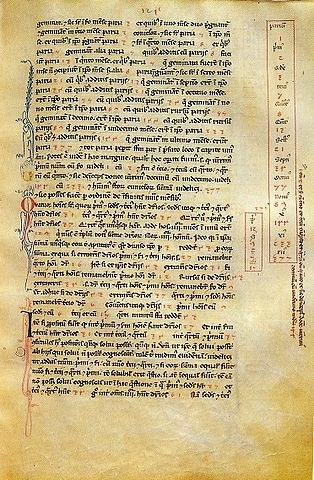
\includegraphics[width=.4\textwidth]{314px-Liber-abbaci-magliab-f124r}
\caption{A page of Fibonacci's Liber Abaci}
\source{Heinz L\"{u}neburg, Leonardi Pisani Liber Abaci oder Lesevergn\"{u}gen eines Mathematikers}
\end{figure}

\section{List of Fibonacci Numbers}

The first 11 Fibonacci numbers $F_n$ for $n = 0, 1, 2, \ldots, 10$ are:

\begin{table}[hbt!]\centering
\caption{First 11 Fibonacci Numbers for $n=0,1,\ldots$}
\begin{tabular}{|c|c|c|c|c|c|c|c|c|c|c|}
\hline
$F_0$ & $F_1$ & $F_2$ & $F_3$ & $F_4$ & $F_5$ & $F_6$ & $F_7$ & $F_8$ & $F_9$ & $F_{10}$\\
\hline
0 & 1 & 1 & 2 & 3 & 5 & 8 & 13 & 21 & 34 & 55 \\
\hline
\end{tabular}
\end{table}

The sequence can also be extended to negative index n using the re-arranged recurrence relation
%
\begin{equation}
F_{n-2} = F_n - F_{n-1},
\end{equation}
%
which yields the sequence of ``negafibonacci'' numbers satisfying
%
\begin{equation}
F_{-n} = (-1)^{n+1} F_n.
\end{equation}
%
Thus the bidirectional sequence is
\begin{table}[hbt!]\centering
\caption{Bidirectional Fibonacci Numbers sequence}
\begin{tabular}{|c|c|c|c|c|c|c|c|c|c|c|}
\hline
$F_{-5}$ & $F_{-4}$ & $F_{-3}$ & $F_{-2}$ & $F_{-1}$ & $F_0$ & $F_1$ & $F_2$ & $F_3$ & $F_4$ & $F_5$ \\\hline
5 & $-3$ & 2 & $-1$ & 1 & 0 & 1 & 1 & 2 & 3 & 5\\\hline
\end{tabular}
\end{table}

\citet{Rohl:1989} gives an account of how Fibonacci numbers can be computed efficiently.

\section{Applications}

\subsection{In Computation}

Fibonacci numbers have wide applications in mathematics as well as computer science:

\begin{itemize}
\item The Fibonacci numbers are important in the computational run-time analysis of Euclid's algorithm to determine the greatest common divisor of two integers: the worst case input for this algorithm is a pair of consecutive Fibonacci numbers.

\item Yuri Matiyasevich was able to show that the Fibonacci numbers can be defined by a Diophantine equation, which led to his original solution of Hilbert's tenth problem.

\item The Fibonacci numbers are also an example of a complete sequence. This means that every positive integer can be written as a sum of Fibonacci numbers, where any one number is used once at most.

\item Moreover, every positive integer can be written in a unique way as the sum of one or more distinct Fibonacci numbers in such a way that the sum does not include any two consecutive Fibonacci numbers. This is known as Zeckendorf's theorem, and a sum of Fibonacci numbers that satisfies these conditions is called a Zeckendorf representation. The Zeckendorf representation of a number can be used to derive its Fibonacci coding.

\item Fibonacci numbers are used by some pseudorandom number generators.

\item Fibonacci numbers are used in a polyphase version of the merge sort algorithm in which an unsorted list is divided into two lists whose lengths correspond to sequential Fibonacci numbers -- by dividing the list so that the two parts have lengths in the approximate proportion $\varphi$. A tape-drive implementation of the polyphase merge sort was described in The Art of Computer Programming.

\item Fibonacci numbers arise in the analysis of the Fibonacci heap data structure.

\item The Fibonacci cube is an undirected graph with a Fibonacci number of nodes that has been proposed as a network topology for parallel computing.

\item A one-dimensional optimization method, called the Fibonacci search technique, uses Fibonacci numbers.

\item The Fibonacci number series is used for optional lossy compression in the IFF 8SVX audio file format used on Amiga computers. The number series compands the original audio wave similar to logarithmic methods such as $\mu$-law.

\item Since the conversion factor 1.609344 for miles to kilometers is close to the golden ratio (denoted $\varphi$), the decomposition of distance in miles into a sum of Fibonacci numbers becomes nearly the kilometer sum when the Fibonacci numbers are replaced by their successors. This method amounts to a radix 2 number register in golden ratio base $\varphi$ being shifted. To convert from kilometers to miles, shift the register down the Fibonacci sequence instead.
\end{itemize}


\subsection{In Nature}

Fibonacci sequences appear in biological settings, in two consecutive Fibonacci numbers, such as branching in trees, arrangement of leaves on a stem, the fruitlets of a pineapple, the flowering of artichoke, an uncurling fern and the arrangement of a pine cone, and the family tree of honeybees. However, numerous poorly substantiated claims of Fibonacci numbers or golden sections in nature are found in popular sources, e.g.,~relating to the breeding of rabbits in Fibonacci's own unrealistic example, the seeds on a sunflower, the spirals of shells, and the curve of waves.

A model for the pattern of florets in the head of a sunflower was proposed by H.~Vogel in 1979. \cite{Vogel:1979} This has the form
\begin{equation}
\theta = \frac{2\pi}{\phi^2} n,\  r = c \sqrt{n}
\end{equation}
where $n$ is the index number of the floret and $c$ is a constant scaling factor; the florets thus lie on Fermat's spiral.

\begin{figure}[hbt!]\centering
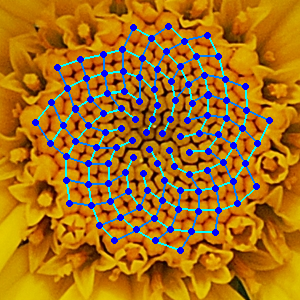
\includegraphics[width=.5\textwidth]{FibonacciChamomile}

\caption{Yellow Chamomile head}
\end{figure}

\chapter{Golden Ratio}

In mathemat
\chapter{Perbincangan, Implikasi dan Cadangan}

\section{Pengenalan}
Bab ini membincangkan dapatan kajian secara menyeluru
\documentclass[12pt]{report}
\usepackage[utf8]{inputenc}
\usepackage{geometry}
\geometry{a4paper, margin=1in}
\usepackage{setspace}
\usepackage{lipsum}
\usepackage{titlesec}
\usepackage{hyperref}
\usepackage{graphicx}
\usepackage{enumitem}

\titleformat{\chapter}[display]
  {\normalfont\huge\bfseries}{\chaptertitlename\ \thechapter}{20pt}{\Huge}

\title{Pembangunan Aplikasi AR Alphabets Prasekolah}
\author{Azhar Manap}
\date{}

\begin{document}

\maketitle
\tableofcontents
\newpage

\chapter{Perbincangan, Implikasi dan Cadangan}

\section{Pengenalan}
Bab ini membincangkan dapatan kajian secara menyeluruh berdasarkan objektif kajian yang telah ditetapkan. Perbincangan ini turut merangkumi implikasi kajian terhadap bidang pendidikan prasekolah, khususnya dalam aspek pengajaran literasi awal menggunakan teknologi Augmented Reality (AR). Selain itu, cadangan bagi kajian lanjutan turut dikemukakan.

\section{Perbincangan Dapatan Kajian}
\subsection{Keberkesanan Aplikasi AR Alphabets terhadap Pencapaian Literasi Awal}
Dapatan menunjukkan bahawa penggunaan aplikasi AR Alphabets telah memberikan impak positif terhadap penguasaan huruf dan fonetik dalam kalangan murid prasekolah...

\subsection{Pengaruh Aplikasi terhadap Tumpuan dan Minat Murid}
Aplikasi AR Alphabets berjaya mengekalkan tumpuan murid dalam jangka masa lebih panjang...

\subsection{Kebolehgunaan Aplikasi oleh Guru dan Murid}
Ujian kebolehgunaan menunjukkan skor tinggi pada Skala Kebolehgunaan Sistem (SUS)...

\section{Implikasi Kajian}
\subsection{Implikasi terhadap Amalan Pengajaran}
Kajian ini menunjukkan bahawa penggunaan teknologi AR bukan sahaja berupaya meningkatkan keberkesanan pengajaran dan pembelajaran...

\subsection{Implikasi terhadap Dasar Pendidikan}
Hasil kajian menyokong pelaksanaan inisiatif transformasi digital dalam pendidikan seperti dalam PPPM 2013–2025...

\subsection{Implikasi terhadap Penyelidikan Masa Hadapan}
Kajian ini membuka ruang kepada lebih banyak kajian lanjutan dalam bidang pembangunan teknologi pendidikan awal kanak-kanak...

\section{Kekuatan dan Kelemahan Kajian}
Kajian ini berjaya membangunkan aplikasi yang berkesan dan diterima baik oleh pengguna...

\section{Cadangan Kajian Lanjutan}
\begin{itemize}
  \item Memperluaskan penggunaan aplikasi ke lebih banyak institusi prasekolah
  \item Membangunkan modul tambahan seperti ejaan dan suku kata
  \item Menyesuaikan aplikasi ke pelantar lain seperti iOS
  \item Mengintegrasikan AI untuk pembelajaran adaptif
\end{itemize}

\section{Penutup}
Bab ini membincangkan dapatan utama kajian dan cadangan penambahbaikan bagi meningkatkan keberkesanan aplikasi dan memperluaskan impaknya.

\end{document}
h berdasarkan objektif kajian yang telah ditetapkan. Perbincangan ini turut merangkumi implikasi kajian terhadap bidang pendidikan prasekolah, khususnya dalam aspek pengajaran literasi awal menggunakan teknologi Augmented Reality (AR). Selain itu, cadangan bagi kajian lanjutan turut dikemukakan.

\section{Perbincangan Dapatan Kajian}
\subsection{Keberkesanan Aplikasi AR Alphabets terhadap Pencapaian Literasi Awal}
Dapatan menunjukkan bahawa penggunaan aplikasi AR Alphabets telah memberikan impak positif terhadap penguasaan huruf dan fonetik dalam kalangan murid prasekolah. Murid dapat mengenal huruf dengan lebih cepat serta memahami bunyi huruf melalui pendekatan interaktif dan visual yang ditawarkan oleh aplikasi tersebut...

\subsection{Pengaruh Aplikasi terhadap Tumpuan dan Minat Murid}
Aplikasi AR Alphabets berjaya mengekalkan tumpuan murid dalam jangka masa lebih panjang...

\subsection{Kebolehgunaan Aplikasi oleh Guru dan Murid}
Ujian kebolehgunaan menunjukkan skor tinggi pada Skala Kebolehgunaan Sistem (SUS)...

\section{Implikasi Kajian}
\subsection{Implikasi terhadap Amalan Pengajaran}
Kajian ini menunjukkan bahawa penggunaan teknologi AR bukan sahaja berupaya meningkatkan keberkesanan pengajaran dan pembelajaran...

\subsection{Implikasi terhadap Dasar Pendidikan}
Hasil kajian menyokong pelaksanaan inisiatif transformasi digital dalam pendidikan seperti dalam PPPM 2013–2025...

\subsection{Implikasi terhadap Penyelidikan Masa Hadapan}
Kajian ini membuka ruang kepada lebih banyak kajian lanjutan dalam bidang pembangunan teknologi pendidikan awal kanak-kanak...

\section{Kekuatan dan Kelemahan Kajian}
Kajian ini berjaya membangunkan aplikasi yang berkesan dan diterima baik oleh pengguna...

\section{Cadangan Kajian Lanjutan}
\begin{itemize}
  \item Memperluaskan penggunaan aplikasi ke lebih banyak institusi prasekolah
  \item Membangunkan modul tambahan seperti ejaan dan suku kata
  \item Menyesuaikan aplikasi ke pelantar lain seperti iOS
  \item Mengintegrasikan AI untuk pembelajaran adaptif
\end{itemize}

\section{Penutup}
Bab ini membincangkan dapatan utama kajian dan cadangan penambahbaikan bagi meningkatkan keberkesanan aplikasi dan memperluaskan impaknya.
ics and the arts, two quantities are in the golden ratio if their ratio is the same as the ratio of their sum to the larger of the two quantities, i.e.~their maximum. The figure on the right illustrates the geometric relationship. Expressed algebraically, for quantities $a$ and $b$ with $a > b$,
\begin{equation}
 \frac{a+b}{a} = \frac{a}{b} \ \stackrel{\text{def}}{=}\ \varphi,
\end{equation}
where the Greek letter $\varphi$ represents the golden ratio. Its value is:
\begin{equation}
\varphi = \frac{1+\sqrt{5}}{2} = 1.61803\,39887\ldots.
\end{equation}

\section{History}

Ancient Greek mathematicians first studied what we now call the golden ratio because of its frequent appearance in geometry. The division of a line into ``extreme and mean ratio'' (the golden section) is important in the geometry of regular pentagrams and pentagons. Euclid's Elements  provides the first known written definition of what is now called the golden ratio: ``A straight line is said to have been cut in extreme and mean ratio when, as the whole line is to the greater segment, so is the greater to the less.'' Euclid explains a construction for cutting (sectioning) a line ``in extreme and mean ratio'', i.e., the golden ratio. (See Figure~\ref{fig:line:golden}.) Throughout the Elements, several propositions (theorems in modern terminology) and their proofs employ the golden ratio.

\begin{figure}[hbt!]\centering
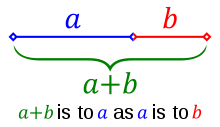
\includegraphics[width=.3\textwidth]{220px-Golden-ratio-line}
\caption{Line segments in the golden ratio}
\label{fig:line:golden}
\end{figure}

\begin{figure}[hbt!]\centering
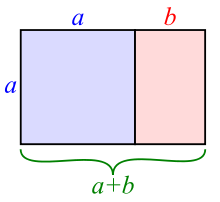
\includegraphics[width=.3\textwidth]{SimilarGoldenRectangles}
\caption{Golden rectangles}
\end{figure}



\section{Calculation}
Two quantities $a$ and $b$ are said to be in the golden ratio $\varphi$ if:
\begin{equation}
 \frac{a+b}{a} = \frac{a}{b} = \varphi.
\end{equation}

One method for finding the value of $\varphi$ is to start with the left fraction. Through simplifying the fraction and substituting in $\frac{b}{a} = \frac{1}{\varphi}$,
\begin{equation}
\frac{a+b}{a} = 1 + \frac{b}{a} = 1 + \frac{1}{\varphi},
\end{equation}

By definition, it is shown that
\begin{equation}
 1 + \frac{1}{\varphi} = \varphi. 
\end{equation}
Multiplying by $\varphi$ gives
\begin{equation*}
\varphi + 1 = \varphi^2
\end{equation*}
which can be rearranged to
\begin{equation*}
{\varphi}^2 - \varphi - 1 = 0.
\end{equation*}
Using the quadratic formula, two solutions are obtained:
\begin{equation*}
\varphi = \frac{1 + \sqrt{5}}{2} = 1.61803\,39887\dots
\end{equation*}
and
\begin{equation*}
\varphi = \frac{1 - \sqrt{5}}{2} = -0.6180\,339887\dots
\end{equation*}
Because $\varphi$ is the ratio between positive quantities $\varphi$ is necessarily positive:
\begin{equation*}
\varphi = \frac{1 + \sqrt{5}}{2} = 1.61803\,39887\dots .
\end{equation*}

Different representations of the golden ratio are given in Table~\ref{tab:goldenratio}.

\begin{table}[hbt!]\centering
\caption{Number representations of the golden ratio}
\label{tab:goldenratio}

\begin{tabular}{|l|l|}
\hline
Form & Representation\\\hline
Binary & 1.1001111000110111011\ldots\\\hline
Decimal & 1.6180339887498948482\ldots\\\hline
Hexadecimal	& 1.9E3779B97F4A7C15F39\ldots\\\hline
Continued fraction & $1 + \cfrac{1}{1 + \cfrac{1}{1 + \cfrac{1}{1 + \cfrac{1}{1 + \ddots}}}}$\\[6ex]\hline
Algebraic form & $\displaystyle\frac{1 + \sqrt{5}}{2}$\\[2ex]\hline
Infinite series & $\displaystyle\frac{13}{8}+\sum_{n=0}^{\infty}\frac{(-1)^{(n+1)}(2n+1)!}{(n+2)!\,n!\,4^{(2n+3)}}$\\[2ex]\hline
\end{tabular}
\end{table}

% rujukan tersenarai dlm refs.bib
\bibliography{refs}

\appendix
% Setiap satu bab apendiks dari fail berasingan
\chapter{Huraian}

Lorem ipsum dolor sit amet, consectetur adipiscing elit. Donec posuere, neque quis feugiat egestas, quam sapien dictum justo, eu vulputate nunc metus sed dui. Integer molestie leo quis libero facilisis, dictum pretium quam ornare. Vestibulum ante ipsum primis in faucibus orci luctus et ultrices posuere cubilia Curae; Vivamus luctus rutrum magna non convallis. Praesent vestibulum consequat eros, et fringilla nisi suscipit id. Nam vulputate justo dui, eu rutrum est accumsan ut. Sed molestie erat vitae mi blandit, in volutpat urna lobortis. Vestibulum mollis rutrum gravida. Fusce dolor nulla, condimentum vel pretium ut, venenatis eget leo. Ut semper placerat mauris, ut tempus est tempor vel. Interdum et malesuada fames ac ante ipsum primis in faucibus. In vitae feugiat diam. Pellentesque accumsan consequat turpis aliquam elementum.

Lorem ipsum dolor sit amet, consectetur adipiscing elit. Donec posuere, neque quis feugiat egestas, quam sapien dictum justo, eu vulputate nunc metus sed dui. Integer molestie leo quis libero facilisis, dictum pretium quam ornare. Vestibulum ante ipsum primis in faucibus orci luctus et ultrices posuere cubilia Curae; Vivamus luctus rutrum magna non convallis. Praesent vestibulum consequat eros, et fringilla nisi suscipit id. Nam vulputate justo dui, eu rutrum est accumsan ut. Sed molestie erat vitae mi blandit, in volutpat urna lobortis. Vestibulum mollis rutrum gravida. Fusce dolor nulla, condimentum vel pretium ut, venenatis eget leo. Ut semper placerat mauris, ut tempus est tempor vel. Interdum et malesuada fames ac ante ipsum primis in faucibus. In vitae feugiat diam. Pellentesque accumsan consequat turpis aliquam elementum.

Lorem ipsum dolor sit amet, consectetur adipiscing elit. Donec posuere, neque quis feugiat egestas, quam sapien dictum justo, eu vulputate nunc metus sed dui. Integer molestie leo quis libero facilisis, dictum pretium quam ornare. Vestibulum ante ipsum primis in faucibus orci luctus et ultrices posuere cubilia Curae; Vivamus luctus rutrum magna non convallis. Praesent vestibulum consequat eros, et fringilla nisi suscipit id. Nam vulputate justo dui, eu rutrum est accumsan ut. Sed molestie erat vitae mi blandit, in volutpat urna lobortis. Vestibulum mollis rutrum gravida. Fusce dolor nulla, condimentum vel pretium ut, venenatis eget leo. Ut semper placerat mauris, ut tempus est tempor vel. Interdum et malesuada fames ac ante ipsum primis in faucibus. In vitae feugiat diam. Pellentesque accumsan consequat turpis aliquam elementum.
\chapter{Perisian}

Lorem ipsum dolor sit amet, consectetur adipiscing elit. Donec posuere, neque quis feugiat egestas, quam sapien dictum justo, eu vulputate nunc metus sed dui. Integer molestie leo quis libero facilisis, dictum pretium quam ornare. Vestibulum ante ipsum primis in faucibus orci luctus et ultrices posuere cubilia Curae; Vivamus luctus rutrum magna non convallis. Praesent vestibulum consequat eros, et fringilla nisi suscipit id. Nam vulputate justo dui, eu rutrum est accumsan ut. Sed molestie erat vitae mi blandit, in volutpat urna lobortis. Vestibulum mollis rutrum gravida. Fusce dolor nulla, condimentum vel pretium ut, venenatis eget leo. Ut semper placerat mauris, ut tempus est tempor vel. Interdum et malesuada fames ac ante ipsum primis in faucibus. In vitae feugiat diam. Pellentesque accumsan consequat turpis aliquam elementum.
\end{document}
\usepackage{longtable}
\usepackage{lscape}
\usepackage[margin=2.5cm]{geometry}
